\documentclass{Vorlage}
%\usepackage[ngerman]{babel}
\usepackage{amsfonts}
\usepackage{graphicx}
\usepackage{url}
\usepackage{amsmath}
\usepackage{adjustbox}
\usepackage{color}
\usepackage{multirow}
\usepackage{bm}
%\usepackage[utf8]{inputenc}
%\bibliographystyle{apalike}
\setlength{\parindent}{0pt}

\pagestyle{fancy}
\renewcommand*\sectionmark[1]{\markboth{\MakeUppercase{#1}}{}}
\begin{document}

\newgeometry{top=2.5cm,bottom=2.0cm,left=2.5cm,right=2.5cm} % Befehl wird nur benötigt, falls Änderungen an den Seitenrändern in der Datei "Vorlage.cls" vorgenommen werden.

\begin{titlepage}

\begin{figure}
 \begin{center}
 
\includegraphics[scale=0.8]{Pictures/logo3}
 \end{center}
\end{figure}
\vspace*{3cm}




\titel{Kleinräumige Extrapolation von Umfragedaten}{}

\vspace{1cm}

\begin{tabular}{p{3.5cm}|p{0.1cm} p{10cm}l}
\textsc{Namen:} & & \textsc{Alexander Lange, Kai Husmann}\\
\textsc{Matr. Nr.:} & & \textsc{21426614}\\
\textsc{Studiengang:} & & \textsc{Angewandte Statistik}\\
\textsc{Mail:} & & \textsc{Alexander.lange$ @ $uni-goettingen.de}\\
\textsc{Kurs:} & & \textsc{Statistisches Praktikum}\\
\textsc{Kursleiter:} & & \textsc{Prof.Dr. Thomas Kneib}\\
\textsc{Lehrstuhl:} & & \textsc{Statistik}\\
\textsc{Fakultät:} & & \textsc{Wirtschaftswissenschaften}\\
\textsc{Abgabedatum:} & & \textsc{30. September 2016}\\
\end{tabular}
\end{titlepage}

\restoregeometry

\pagenumbering{Roman} % \pagenumbering{roman} = Kleinschreibung: II -> ii.

\pagestyle{plain}

\tableofcontents % Inhaltsverzeichnis.

\newpage % Neue Seite.

\listoffigures % Abbildungsverzeichnis.

\listoftables % Tabellenverzeichnis.

\newpage

\pagenumbering{arabic} % Ab hier folgt die arabische Seitennummerierung.

%\renewcommand{\thesection}{\arabic{section}} % Römische Nummerierung der Kapitelüberschriften.

%============================================ Instroduction ========================================================%
\pagestyle{fancy}

\section{Einleitung}

\newpage

%=================================================== Main Part  ====================================================%
\section{Material und Methoden}
\section{Daten}
Insgesamt liegen für die Analysen drei Umfragen vor. Die kleinste Datei enthält Angaben zur Bewertung der Wohngegend, der Meinung zu Stutttgart 21 sowie weitere sozioökonomische Kovariablen, die zur Erklärung der beiden unabhängigen Variablen dienen. Diese Datei wird im Folgenden als Stichprobe bezeichnet. Die Bevölkerung Stuttgarts bildet die Grundgesamtheit dieser Unteruchung. Da die Zensus Umfrage von 20?? und die Bürgerumfrage von 20?? dieseer Grundgesamtheit sehr nah kommen, wird angenommen, dass diese beiden Umfragen jeweils die Grundgesamtheit repräsentieren.




\subsection{Deskriptive Statistik}

In diesem Kapitel soll der Stichprobendatensatz vorgestellt werden, sowie ein kurzer Einblick in die beiden Datensätze zur Grundgesamtheit der Bevölkerung von Stuttgart gegeben werden. Anhand des Stichprobendatensatzes soll im Verlauf der Arbeit das Modell zur Extrapolation geschätzt werden und mit Hilfe der Datensätze zur Grundgesamtheit die Häufigkeiten der abhängigen Variablen prognostiziert werden. \\
Tabelle \ref{Datensatz} gibt einen Überblick über den Inhalt der Stichprobe. Wie zu erkennen ist, handelt es sich dabei um strukturell sozioökonomische Variablen. Zudem enthält der Datensatz drei verschiedene räumliche Informationen zu den Beobachtungen, auf die im nächsten Kapitel ausführlicher eingegangen wird.\\

\begin{table}[h]
\centering
\caption{Datensatz}
\label{Datensatz}
\adjustbox{max height=\dimexpr\textheight-5.5cm\relax,
           max width=\textwidth}{
\begin{tabular}{l|c|c}
\multicolumn{2}{l}{Anzahl Beobachtungen: 3.143}     \\ \hline \hline
\textbf{Variable} & \textbf{Mögliche Ausprägungen} & \textbf{Modellierung} \\ \hline
Bewertung Wohngegend &  6 & Geordnet Kategorial \\ \hline
Meinung Stuttgart 21 &  6 & Geordnet Kategorial \\ \hline
Personenanzahl im Haushalt & 5 & Nicht Parametrisch \\ \hline
Monatliches Netto Haushaltseinkommen & 6 & Nicht Parametrisch \\ \hline
Altersklasse Befragter & 6 & Nicht Parametrisch \\ \hline
Geschlecht & 2 & Parametrisch\\ \hline
Familienstand & 4 & Parametrisch \\ \hline
Nationalität & 2 & Parametrisch \\ \hline
Stadtbezirk & 23 & Markov-Zufallsfeld \\ \hline 
Stadtteil &  142 & Markov-Zufallsfeld \\ \hline 
Gauß-Krüger & & Tensorprodukt-Splines  \\ \hline \hline
\end{tabular}
}
\end{table}

Die rechte Spalte zeigt an, wie die einzelnen Variablen in das zu schätzende Modell einfließen sollen. Dabei ist zu erkennen, dass nominal skalierte Variablen, wie z.B. Nationalität als parametrisch und metrisch skalierte Variablen wie z.B. die Altersklasse der Befragten als nicht parametrisch modelliert werden sollen \cite[p. 9]{fahrmeir2009regression}. Genauere Erläuterungen zur Modellierung der Variablen finden sich im Kapitel Methodik. Die beiden Datensätze zur Grundgesamtheit stammen aus einer Bürgerumfrage mit 470.190 Beobachtungen und dem Zensus mit 380.238 Beobachtungen. Im Verhältnis zu den Grundgesamtheiten  dieser Größenordnung sind 3143 Beobachtungen in der Stichprobe relativ gering, was eine gewisse Unsicherheit für die Extrapolation mit sich bringt [...].\\
Weiterhin ist zu beachten, dass Informationen zu dem monatlichen Netto Haushaltseinkommen in beiden Grundgesamtheiten fehlen und somit die Variable nicht für die Prognose verwendet werden kann. Auch war eine denkbare Erstellung von Proxy-Variablen nicht möglich. Eine genaue Auflistung der enthaltenen Variablen aus den Grundgesamtheiten ist im Anhang verfügbar. Die Arbeit zielt darauf ab, die Meinung der Befragten zu dem Projekt Stuttgart 21 und die Zufriedenheit mit der Wohngegend der Befragten auf die Grundgesamtheit zu extrapolieren. Daher ist es sinnvoll die Ausprägungen dieser Variablen genauer zu untersuchen.\\
Dazu wurde Abbildung \ref{endogene} erstellt. Sie zeigt die Häufigkeiten der einzelnen Ausprägungen der beiden endogenen Variablen. Wie schon zuvor aus Tabelle \ref{Datensatz} ersichtlich, besitzen beide Variablen sechs mögliche Realisationen, wobei die Klasse \textit{keine Angabe} keine Informationen über die Meinung der Befragten liefert und diese Beobachtungen daher aus dem Datensatz entfernt werden müssen. Damit bleiben fünf mögliche Klassen zur Modellierung übrig.

\begin{figure}[h]
 \begin{center}
 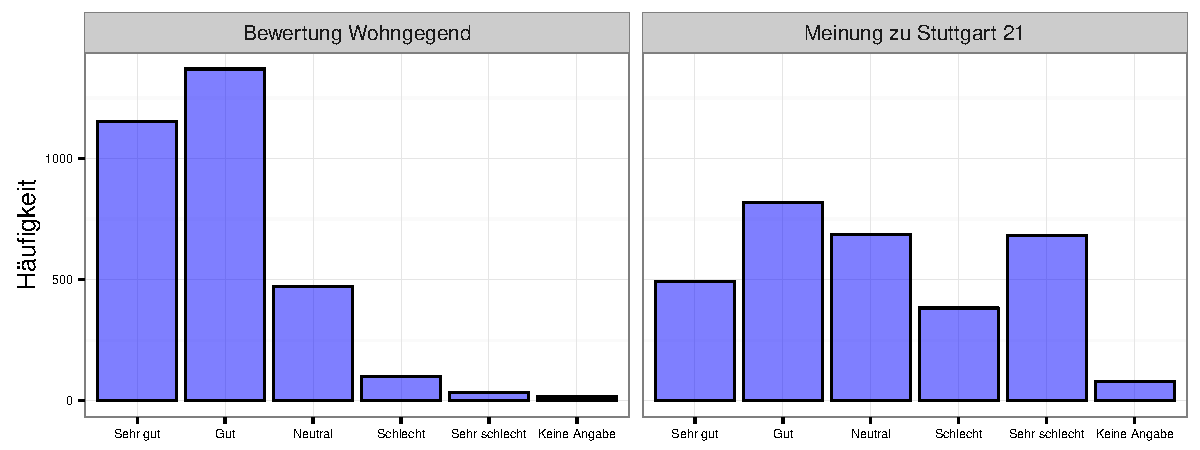
\includegraphics[scale=0.8]{Pictures/BarResp}
 \caption{Endogene Variablen}
 \label{endogene}
 \end{center}
\end{figure}

Aus Abbildung \ref{endogene} ist zudem ersichtlich, dass die Verteilungen der Beiden Variablen sehr verschieden sind für die gleichen Antwortmöglichkeiten. Während die meisten befragten Personen ihre Wohngegend mit \textit{gut} oder \textit{sehr gut} bewertet haben, sind die Antworten zum Projekt Stuttgart 21 eher gleichmäßig verteilt.\\
Abschließend ist die Entscheidung gefallen die Bewertung der Wohngegend mit fünf Klassen zu Modellieren, um eine möglichst genau Prognose der Meinung der Bevölkerung zu erreichen. Zudem sind keinerlei Daten zur Bewertung der Wohngegend für die Grundgesamtheit verfügbar, womit auch keine Rücksicht auf eine mögliche Validierung des Modells genommen werden muss. Hingegen ist eine Validierung für die Meinung zu Stuttgart 21 mit den Ergebnissen der Volksabstimmung aus dem Jahre 2011 möglich \cite{Amt}. Allerdings bietet die Volksabstimmung nur Informationen für maximal drei Kategorien (\textit{Zustimmung}, \textit{Ablehnung}, \textit{Enthaltung}), weshalb die weitere Analyse ebenfalls mit drei Kategorien erfolgen soll. Dafür werden die Kategorien \textit{sehr gut} und \textit{Gut} zusammengefasst zu \textit{Zustimmung} und die Klassen \textit{schlecht} und \textit{sehr schlecht} zu \textit{Ablehnung}. Die Klasse \textit{neutral} soll als mittlere Kategorie erhalten bleiben. 
Für die exogen in die Analyse einfließenden Variablen sind detailliertere Informationen zu den Häufigkeiten der Ausprägungen im Anhang verfügbar. 

\newpage

\subsection{Räumliche Effekte}

Da in dieser Arbeit ein besonderer Schwerpunkt auf die unterschiedlichen räumlichen Effekte gelegt werden soll, vergleicht dieses Kapitel alle drei räumlichen Effekte für beide endogene Variablen. Zunächst wird der stetige räumliche Effekt mit den Gauss-Krüger Informationen behandelt. Anschließend folgen die diskreten räumlichen Informationen auf Bezirks und Stadtteilebene.\\
Aus Abbildung \ref{XYStuttgart3} ist die absolute Häufigkeit der Beobachtungen für jede der drei Kategorien zur Meinung zu Stuttgart 21 ersichtlich. Zuerst ist erkenntlich wo die meisten Personen befragt wurden, nämlich in der nähe des Innenstadt Bereichs. Hier findet sich eine Häufung der Beobachtung zu allen drei Kategorien, wohingegen die Randbezirke im allgemeinen weniger Beobachtungen aufweisen. Außerdem ist zu sehen, dass auf Grund der geographischen Beschaffenheit der Region in einigen Bereichen mit weniger Beobachtungen zu rechnen ist z.B. beim Wald im Westen und der hügeligen Landschaft im Osten.    

\begin{figure}[h]
 \begin{center}
 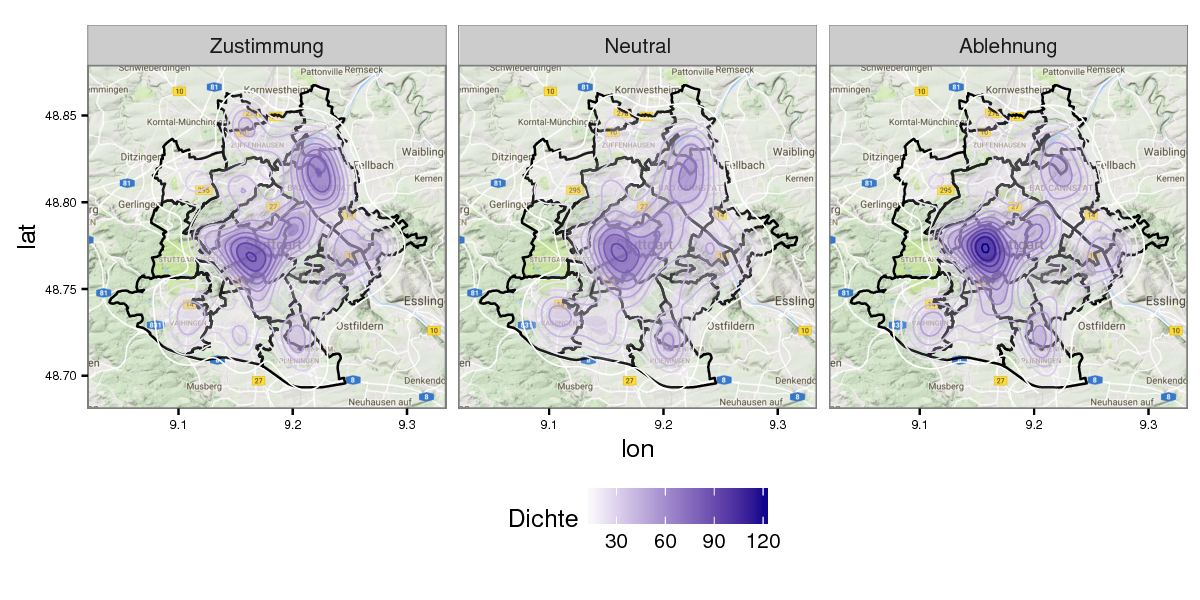
\includegraphics[scale=0.8]{Pictures/XYStuttgart3.png}
 \caption{Gauss Krüger Informationen Stuttgart 21}
 \label{XYStuttgart3}
 \end{center}
\end{figure}

Zu der spezifischen Häufung der Beobachtungen innerhalb der Klassen ist ein leichter Trend zu erkennen, sodass für die Kategorie \textit{Zustimmung} eine größere Häufung der Beobachtungen im Nordosten zu erkennen ist. Für die Kategorie \textit{Ablehnung} ist eher noch eine stärkere Konzentration auf den Bereich Südwestlich der Innenstadt zu erkennen und einige kleinere Häufung im Süden Stuttgarts. Die Beobachtungen der Kategorie \textit{neutral} sind eher gleichmäßig über die Stadt verteilt.\\
Abbildung \ref{XYWohnG5} zeigt die Absolute Verteilung der Beobachtungen für die fünf Kategorien zur Bewertung der Wohngegend. Hier zeigt sich ein deutlich heterogenes Bild als bei der Meinung zu Stuttgart 21. Die Beobachtungen der Klasse \textit{Sehr gut} häufen sich sehr stark im Innenstadt Bereich und im Süden. Die Kategorie \textit{gut} verteilt sich über das gesamte Stadtgebiet mit einer stärkeren Konzentration in der Innenstadt und im Nordosten. Für die Klasse \textit{Neutral} zeigt sich schon eine stärkere Konzentration auf den Osten und Nordosten der Stadt im Vergleich zu den beiden vorherigen Klassen. Am interessantesten ist hier ist die Lokalisierung der Personen die ihre Wohngegend mit \textit{schlecht} oder \textit{sehr schlecht} bewertet haben. Hier finden sich nahezu alle Beobachtungen im Osten und Nordosten Stuttgarts.

\begin{figure}[h]
 \begin{center}
 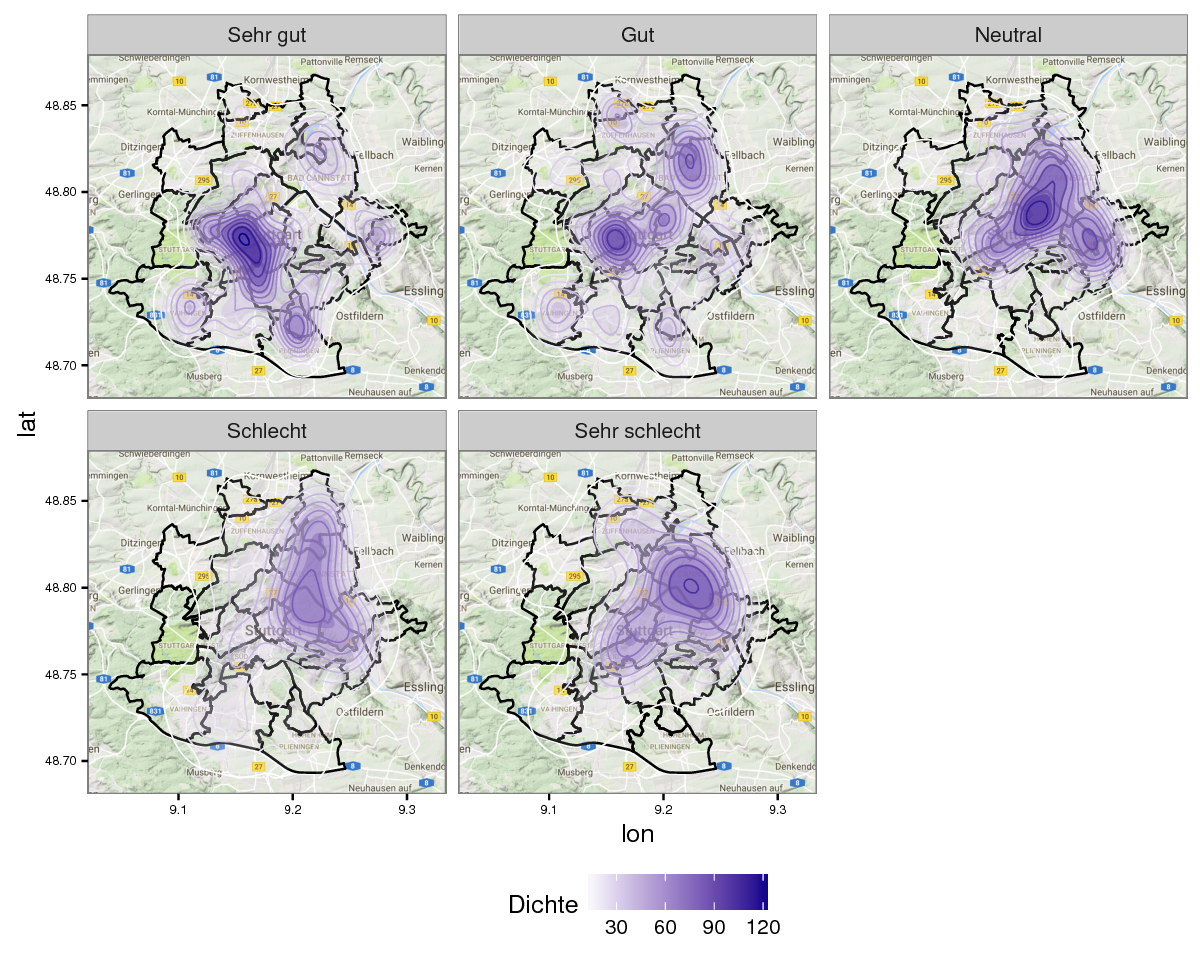
\includegraphics[scale=0.8]{Pictures/XYWohnG5.png}
 \caption{Gauss Krüger Informationen Bewertung Wohngegend}
 \label{XYWohnG5}
 \end{center}
\end{figure}

Allerdings ist auch zu beachten, dass der Anteil der Personen, die ihre Wohngegend mit \textit{schlecht} oder \textit{sehr schlecht} bewertet haben sehr gering ist im Vergleich zu allen Befragten wie aus Abbildung \ref{endogene} ersichtlich.\\
Als nächstes können die diskreten räumlichen Informationen auf Stadtbezirksebene untersucht werden. Dazu wurde Abbildung \ref{BStuttgart21} erstellt. Hier sind die Anteile der drei Klassen für die jeweiligen Bezirke zu erkennen. Zu sehen ist, dass der Anteil der Personen die das Projekt Stuttgart 21 positiv bewerten in allen Stadtbezirken relativ hoch ist, wobei der Anteil in den nordöstlichen Bezirken etwas höher ist. Die neutrale Klasse hat in alles Bezirken einen eher geringeren Anteil und es ist kein deutliches Muster von höheren oder niedrigeren Anteilen erkennbar. Die Klasse \textit{Ablehnung} hat etwas höhere Anteile in den mittleren und südlichen Bezirken. Insgesamt deckt sich das Bild der Anteile auf Bezirksebene mit den absoluten Häufigkeiten aus Abbildung \ref{XYStuttgart3}. Die Anteile auf Bezirksebene mit fünf Klassen für die Bewertung der Wohngegend sind im Anhang verfügbar. Zu beachten ist hier, dass die Anteile auf fünf verschiedenen Skalen dargestellt werden, da der Anteil der beiden negativen Klassen zu gering ist im Verhältnis zu den positiven Klassen, um sie anders darzustellen. Aber auch hier deckt sich die Verteilung der hohen und niedrigen Anteile mit den Absoluten Anzahlen an Beobachtungen aus Abbildung \ref{XYWohnG5}.

\begin{figure}[h]
 \begin{center}
 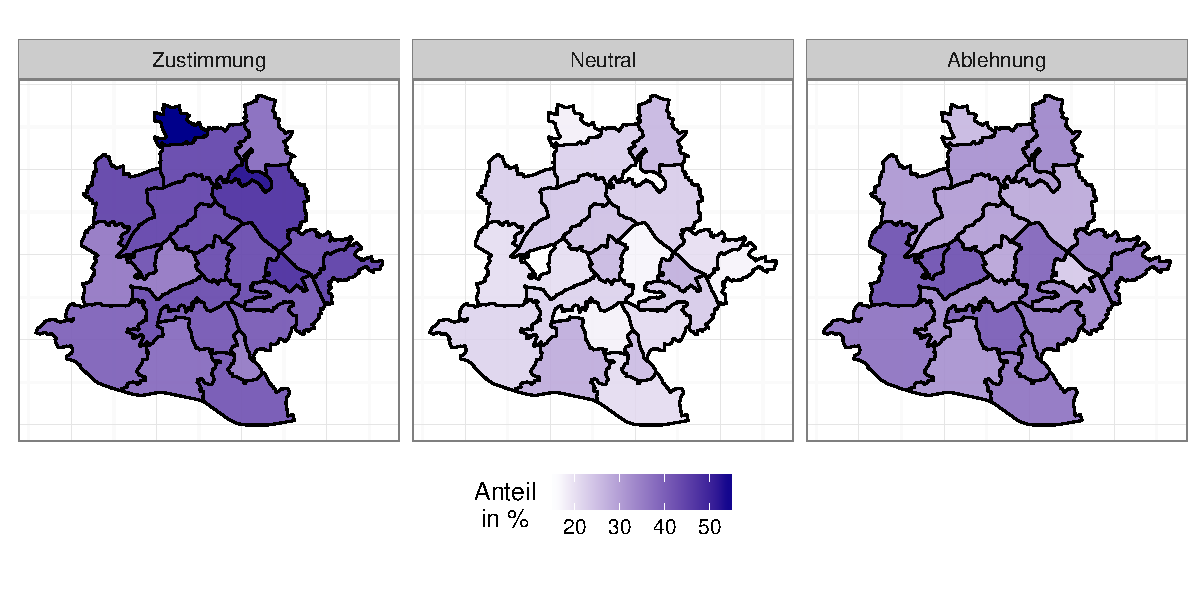
\includegraphics[scale=0.8]{Pictures/BStuttgart3}
 \caption{Anteile in Bezirken Stuttgart 21}
 \label{BStuttgart21}
 \end{center}
\end{figure}

Die letzte räumliche Information ist der Anteil der jeweiligen Klasse pro Stadtteil. Wie schon aus Tabelle \ref{Datensatz} bekannt, besitzt die Stadtteilebene eine wesentlich feinere Aufteilung, als die Bezirksebene. Dadurch ist es möglich, dass in einzelnen Stadtteilen keine Beobachtungen einer Klasse auftauchen. Damit kann die Ansicht auf Stadtteilebene zu einer Überschätzung der Bedeutung einer bestimmten Klasse in einem Stadtteil führen. Die Anteile der drei Klassen zu der Meinung zu Stuttgart 21 sind aus Abbildung \ref{SStuttgart21} zu entnehmen.

\begin{figure}[h]
 \begin{center}
 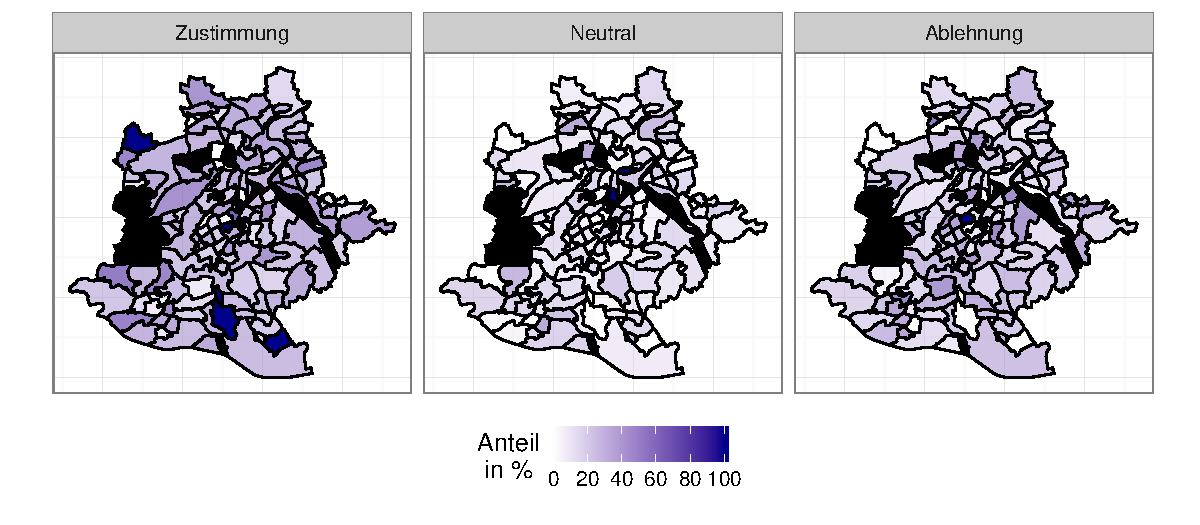
\includegraphics[scale=0.8]{Pictures/SStuttgart3}
 \caption{Anteile in Stadtteilen Stuttgart 21}
 \label{SStuttgart21}
 \end{center}
\end{figure}

Die schwarz eingefärbten Flächen signalisieren Stadtteile in denen von keiner der drei Klasse eine Beobachtung vorhanden sind. Wie bereits erwähnt handelt es dich dabei vor allem um Regionen die auf Grund ihrer geographischen Beschaffenheit kaum Einwohner haben (z.B. Wald). Hier fügt sich das Bild der Anteile nicht ganz in den bisherigen Verlauf der räumlichen Statistiken ein. In keiner der drei Klassen lässt sich klar eine Struktur oder räumliche Korrelation der Stadtteile beobachten. Die Anteile auf Stadtteileebene zu der Bewertung der Wohngegend sind im Anhang verfügbar, wobei die Plots wieder mit eigenen Skalen illustriert wurden. Hier zeigt sich ein ähnlich unklares Muster wie bei der Meinung zu Stuttgart 21.\\
Insgesamt ist zu sagen, dass die Gauss-Krüger Informationen ein relativ klaren Einblick in die Verteilung der Beobachtungen in der jeweiligen Klasse geben. Bei den diskreten räumlichen Informationen könnte die grobe Aufteilung auf Bezirksebene zu einem Underfitting und die sehr feine Aufteilung auf Stadtteilebene zu einem Overfitting führen [...]. Zudem ist zu vermuten, dass die räumlichen Informationen einen stärkeren Effekt auf die Bewertung der Wohngegend haben, als auf die Meinung zu Stuttgart 21.

\section{Statistische Methoden}

\subsection{Modell}
Kurze Erläuterung GAM und logit,... Zusammengesetzt aus parametrischen Effekten und Splines

\subsection{Modellwahl}
Basierend auf den vorhergegangenen Analysen des Beamten- und Eigenheimanteils in Stuttgart wurde die R Funktion \texttt{stepAIC()} zur schrittweisen AIC (CITE AKAIKE) Berechnung programmiert, die zur Identifikation der geeignetsten Kovariablenkombination dient. In der Funktion werden mithilfe der \texttt{gam()} Funktion des \texttt{mgcv} CITE WOOD 2011 Paketes generaliserte additive Modelle mit unterschiedlichen Kovariablen erstellt und deren AIC berechnet. Vor dem Aufruf der Funktion müssen die abhängige Variable, die Verteilungsannahme des Regressionsmodelles, die Gewichtungen der Einzelbeobachtungen und unveränderliche Kovariablen definiert werden. Außerdem muss eingeschätzt werden, welche der veränderlichen Kovariablen parametrisch oder semiparametrisch als Spline in das Modell eingehen. Es wird zunächst der AIC des einfachsten, nur aus den fest vorgegebenen Kovariablen bestehenden Modells berechnet. In Iteration 1 werden alle veränderlichen Kovariablen einzeln nacheinander in die Modellformel aufgenommen und es wird jeweils ein GAM erstellt sowie dessen AIC berechnet. Die Kovariablen gehen entsprechend der vorigen Eingabe parametrisch oder semiparametrisch ein. Falls die Hinzunahme mindestens einer Kovariablen in Iteration 1 zu einer Reduktion des AIC führt, wird diejenige Kovariable, welche zum Modell mit dem kleinsten AIC führt zur Modellformel hinzugefügt. Falls das Modell nur mit den festen Modellbestandteilen bereits den geringsten AIC zeigt ist die Modellwahl folglich in Iteration 1 bereits beendet.\\ Andernfalls setzt sich das Ausgangsmodell für Iteration 2 aus den festen Kovariablen und einer weiteren Kovariable zusammen. In Iteration 2 werden wie zuvor alle verbleibenden Kovariablen zunächst nacheinander zur aktuellen Modellformel hinzugefügt. Wenn die Kovariable mit dem geringsten AIC gefunden ist (falls diese existiert und das Modell aus Iteration 1 nicht bereits das geeignetste ist), werden alle veränderbaren Kovariablen in Iteration 2 nochmals nacheinander eliminiert. Das Modell mit dem geringsten AIC bildet das Ausgangsmodell der nächsten Iteration. Dies wird wiederholt bis in einer Iteration kein Modell mit einem geringeren AIC als in der vorigen Iteration parametrisiert werden kann. Um die Laufzeit der Funktion zu begrenzen, wurde auf die Analyse von Wechselwirkungen zwischen den Kovariablen verzichtet. Wechselwirkungen können jedoch als unveränderliche Modellbestandteile eingehen.

\subsection{Evaluierung}

\section{Ergebnisse}

% Please add the following required packages to your document preamble:
% \usepackage{multirow}
\begin{table}[h]
\centering
\caption{Validierung}
\label{vali}
\begin{tabular}{llll|cc|cc}
\hline \hline
                        &                               &                          &   & \multicolumn{2}{c|}{MSE} & \multicolumn{2}{c}{Überdeckungswk.} \\
                        &                               &                          &   & Zustimmung  & Ablehnung  & Zustimmung        & Ablehnung       \\ \hline
\multirow{12}{*}{3 Kl.} & \multirow{4}{*}{Gauss-Krüger} & \multirow{2}{*}{Bez.}    & U & 0.04       & 0.749      & 1                 & 0.043           \\
                        &                               &                          & Z & 0.116       & 0.557      & 0.391             & 0               \\ \cline{3-8} 
                        &                               & \multirow{2}{*}{Sadtt.}  & U & 0.461       & 5.708      & 0.954             & 0.139           \\
                        &                               &                          & Z & 0.813       & 4.415      & 0.553             & 0.02            \\ \cline{2-8} 
                        & \multirow{4}{*}{Bezirke}      & \multirow{2}{*}{Bez.}    & U & 0.041       & 0.756      & 1                 & 0.043           \\
                        &                               &                          & Z & 0.117       & 0.562      & 0.522             & 0               \\ \cline{3-8} 
                        &                               & \multirow{2}{*}{Stadtt.} & U & 0.482       & 5.678      & 0.934             & 0.139           \\
                        &                               &                          & Z & 0.835       & 4.38       & 0.567             & 0.027           \\ \cline{2-8} 
                        & \multirow{4}{*}{Stadtteile}   & \multirow{2}{*}{Bez.}    & U & 0.023       & 0.903      &                   &                 \\
                        &                               &                          & Z & 0.081       & 0.593      &                   &                 \\ \cline{3-8} 
                        &                               & \multirow{2}{*}{Stadtt.} & U & 0.453       & 6.69       &                   &                 \\
                        &                               &                          & Z & 0.61        & 4.641       &                   &                 \\ \hline
\multirow{8}{*}{2 Kl.}  & \multirow{4}{*}{Gauss-Krüger} & \multirow{2}{*}{Bez.}    & U & 0.337       & 0.337      &                   &                 \\
                        &                               &                          & Z & 0.164      & 0.164      &                   &                 \\ \cline{3-8} 
                        &                               & \multirow{2}{*}{Stadtt.} & U & 2.87       & 2.87      &                   &                 \\
                        &                               &                          & Z & 1.65       & 1.65      &                   &                 \\ \cline{2-8} 
                        & \multirow{4}{*}{Bezirke}      & \multirow{2}{*}{Bez.}    & U & 0.337       & 0.337      &                   &                 \\
                        &                               &                          & Z & 0.164       & 0.164      &                   &                 \\ \cline{3-8} 
                        &                               & \multirow{2}{*}{Stadtt.} & U & 2.87        & 2.85      &                   &                 \\
                        &                               &                          & Z & 1.65        & 1.64     &                   &                 \\ \hline \hline
\end{tabular}
\end{table}

%\clearpage
%============================================== Conlcusion =========================================================%

\section{Fazit}

\clearpage


%============================================ References ===========================================================%
\addcontentsline{toc}{section}{\numberline{}Literatur}
\bibliographystyle{apalike}
\bibliography{LiteraturStuttgart.bib} 

%\section{References}
%\renewcommand{\section}[2]{}
%\addcontentsline{toc}{section}{References}
%\renewcommand{\bibname}{4 References}
%\phantomsection
%\addcontentsline{toc}{section}{References}




\clearpage

%============================================== Appendix ============================================================%
%\appendix
%\pagestyle{Myheadings}
\chead{ANHANG}
%\pagestyle{}
%\section{$A^{-1}$ Appendix}
%\setcounter{secnumdepth}{0}

\begin{appendix}

\section*{Anhang}
\addcontentsline{toc}{section}{\numberline{}Anhang}


\begin{table}[h]
\centering
\caption{Grundgesamtheit Bürgerumfrage}
\adjustbox{max height=\dimexpr\textheight-5.5cm\relax,
           max width=\textwidth}{
\begin{tabular}{l|c|c}
\multicolumn{3}{l}{Anzahl Beobachtungen: 470.190}     \\ 
\hline \hline
\textbf{Variable} & \textbf{Modellierung} & \textbf{Mögliche Ausprägungen}  \\ \hline
\multicolumn{1}{l|}{Altersklasse} &  Nicht Parametrisch & 14 \\ \hline
\multicolumn{1}{l|}{Geschlecht} &  Parametrisch  & 2 \\ \hline
\multicolumn{1}{l|}{Nationalität} & Parametrisch  & 2 \\ \hline
\multicolumn{1}{l|}{Familienstand} & Parametrisch & 4 \\ \hline
\multicolumn{1}{l|}{Haushaltsgröße} &  Nicht Parametrisch  & 5 \\ \hline
\multicolumn{1}{l|}{Wohndauer} & Nicht Parametrisch  & 3 \\ \hline
\multicolumn{1}{l|}{ALG II Quote} & Nicht Parametrisch  & 9 \\ \hline
\multicolumn{1}{l|}{Ein/Zweifamilienhäuser}& Nicht Parametrisch & 8 \\ \hline 
\multicolumn{1}{l|}{Gauß-Krüger} & Tensorprodukt-Splines & \\ \hline \hline
\end{tabular}

}
\end{table}

\begin{table}[h]
\centering
\caption{Grundgesamtheit Zensus}
\adjustbox{max height=\dimexpr\textheight-5.5cm\relax,
           max width=\textwidth}{
\begin{tabular}{l|c|c}
\multicolumn{3}{l}{Anzahl Beobachtungen: 380.238}     \\ 
\hline \hline
\textbf{Variable} & \textbf{Modellierung} & \textbf{Mögliche Ausprägungen}  \\ \hline
\multicolumn{1}{l|}{Altersklasse} &  Nicht Parametrisch & 9 \\ \hline
\multicolumn{1}{l|}{Geschlecht} & Parametrisch  & 2 \\ \hline
\multicolumn{1}{l|}{Nationalität} & Parametrisch  & 2 \\ \hline
\multicolumn{1}{l|}{Familienstand} & Parametrisch & 4 \\ \hline
\multicolumn{1}{l|}{Haushaltsgröße} &  Nicht Parametrisch  & 6 \\ \hline
\multicolumn{1}{l|}{Wohnfläche} & Nicht Parametrisch & 24 \\ \hline
\multicolumn{1}{l|}{Stellung Beruf} & Parametrisch  & 9 \\ \hline
\multicolumn{1}{l|}{Beamter}& Parametrisch & 2 \\ \hline 
\multicolumn{1}{l|}{Gebäudetyp}& Parametrisch & 10 \\ \hline
\multicolumn{1}{l|}{Gebäudenutzung}& Parametrisch & 2 \\ \hline
\multicolumn{1}{l|}{Gauß-Krüger} & Tensorprodukt-Splines & \\ \hline \hline
\end{tabular}

}
\end{table}

\begin{figure}[h]
 \begin{center}
 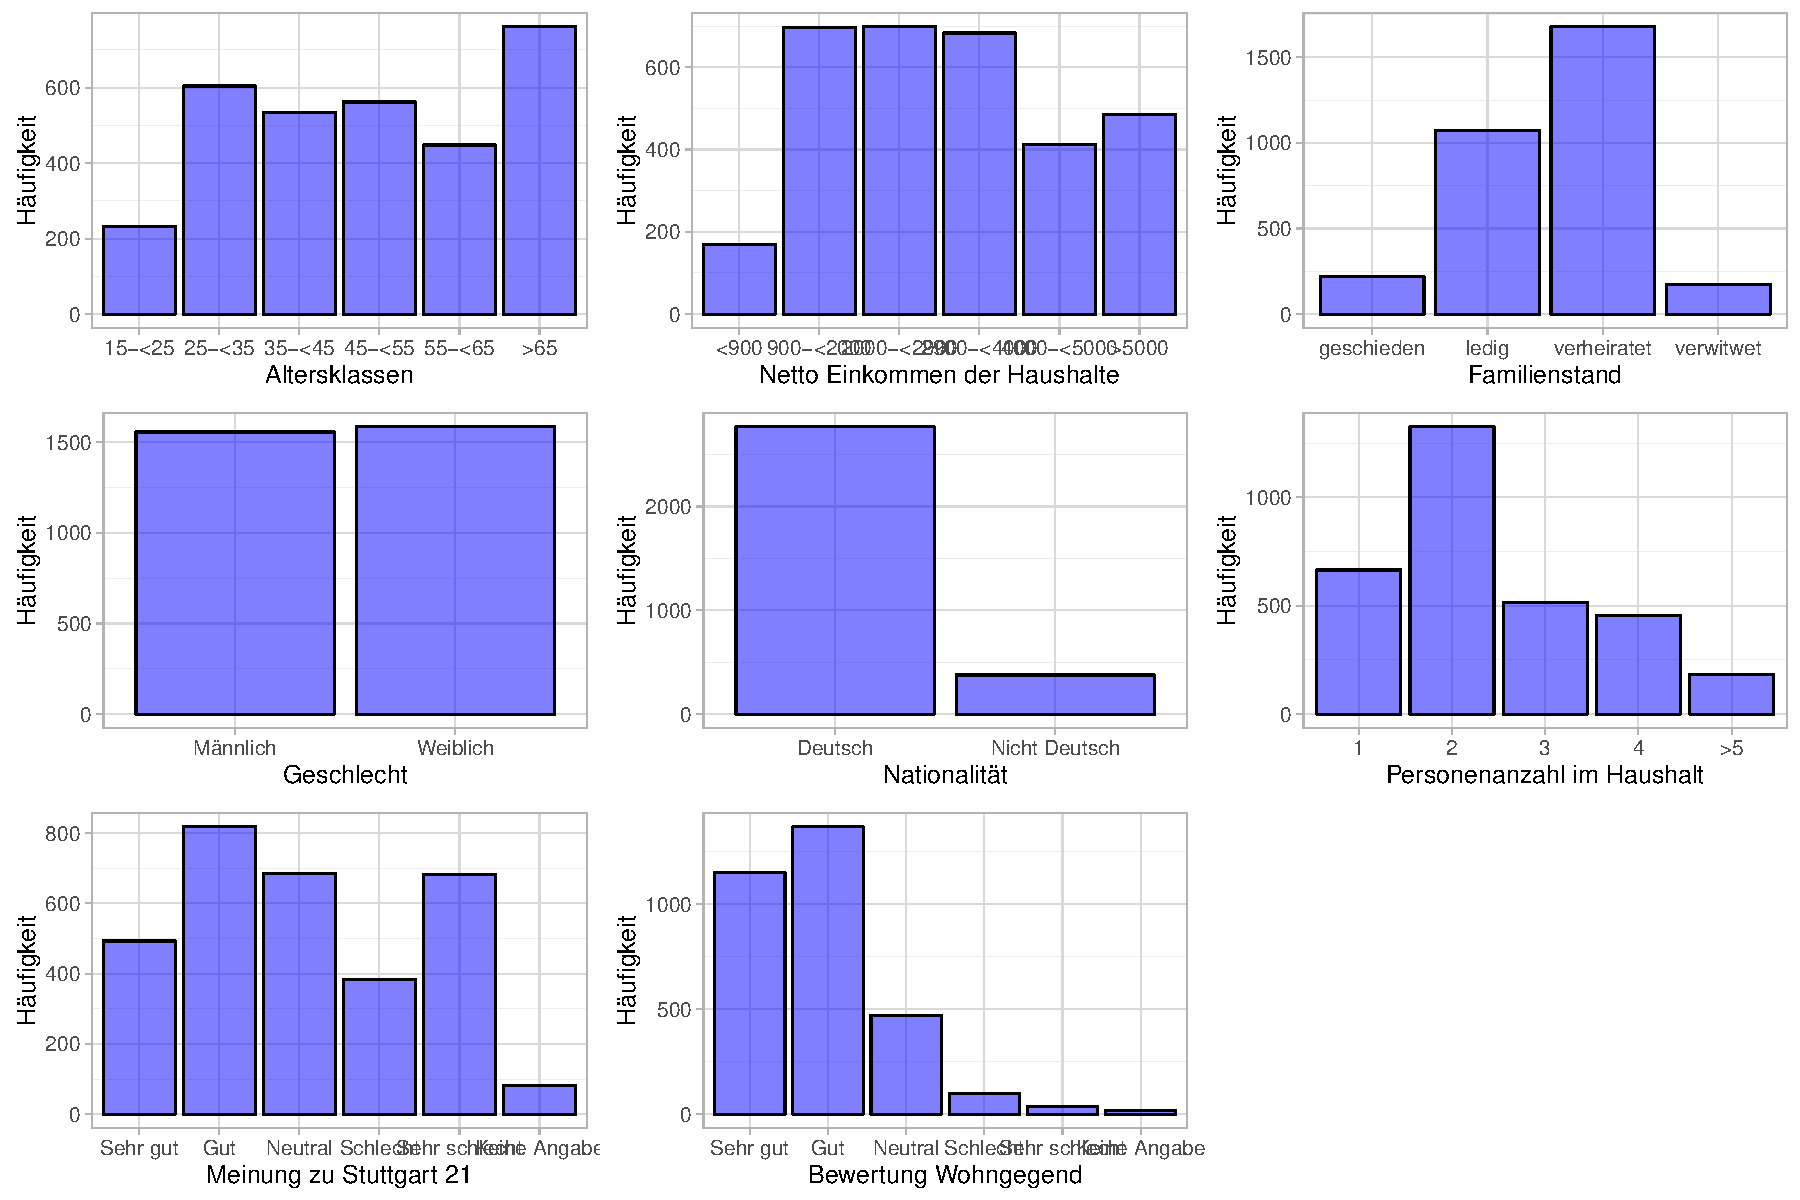
\includegraphics[scale=0.8]{Pictures/BarData}
 \end{center}
\end{figure}


\begin{figure}[h]
 \begin{center}
 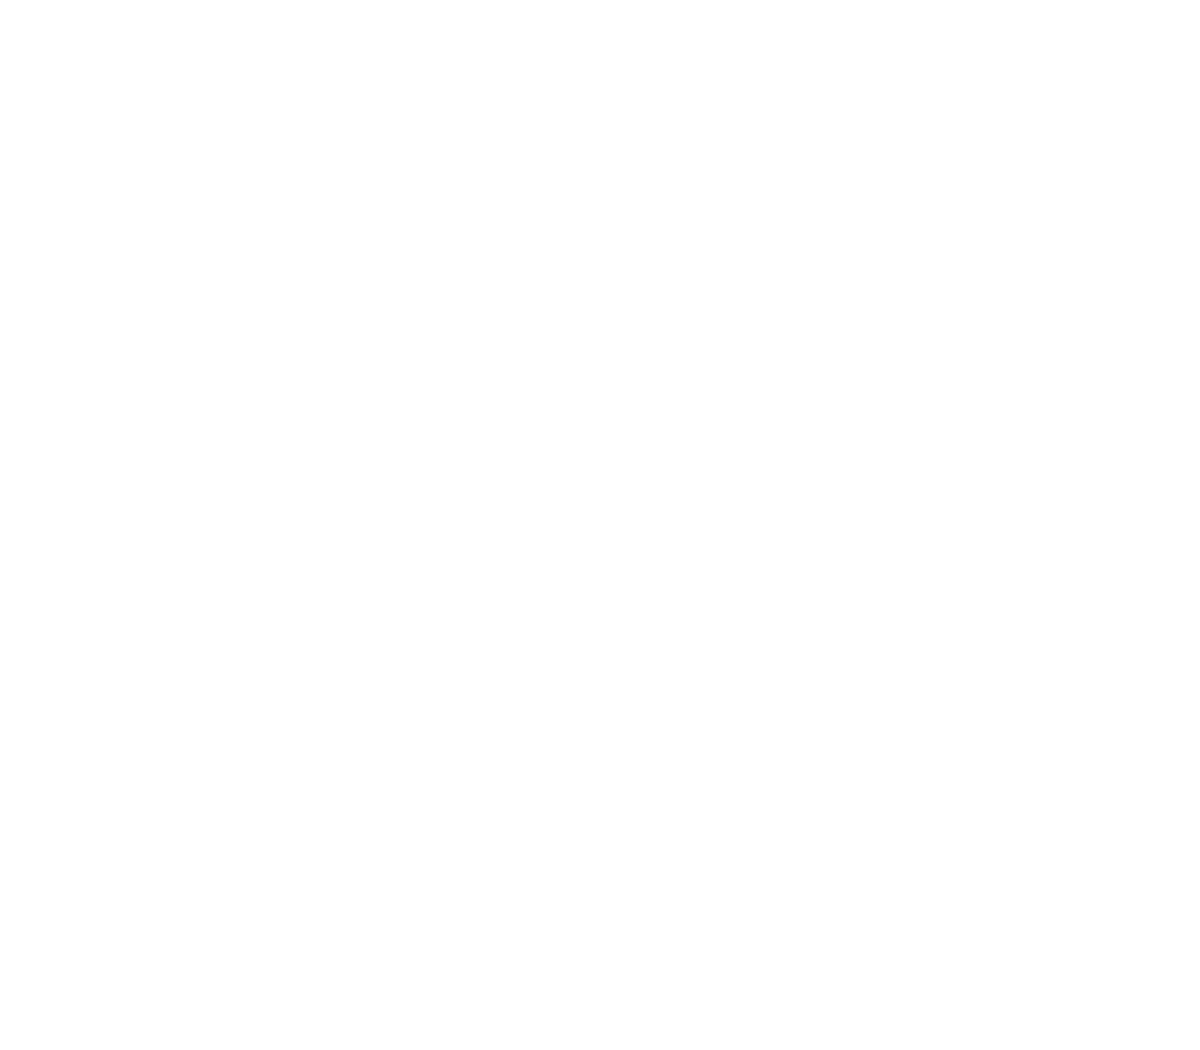
\includegraphics[scale=0.8]{Pictures/BWohn}
 \caption{Anteile in Bezirken Bewertung Wohngegend}
 \label{BWohn}
 \end{center}
\end{figure}

\begin{figure}[h]
 \begin{center}
 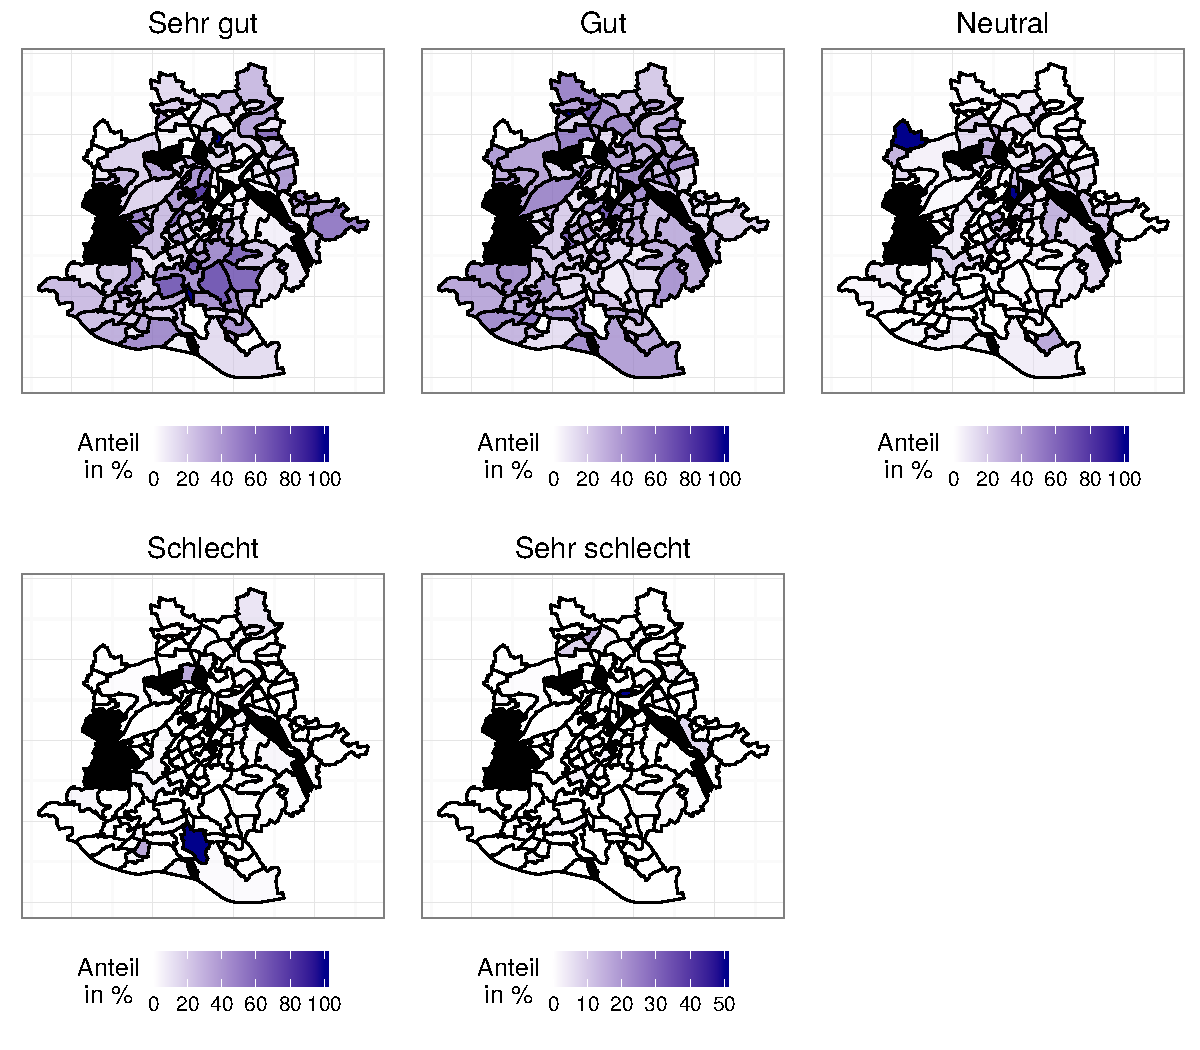
\includegraphics[scale=0.8]{Pictures/SWohn}
 \caption{Anteile in Stadtteilen Bewertung Wohngegend}
 \label{SWohn}
 \end{center}
\end{figure}

%\begin{figure}[h]
% \begin{center}
% 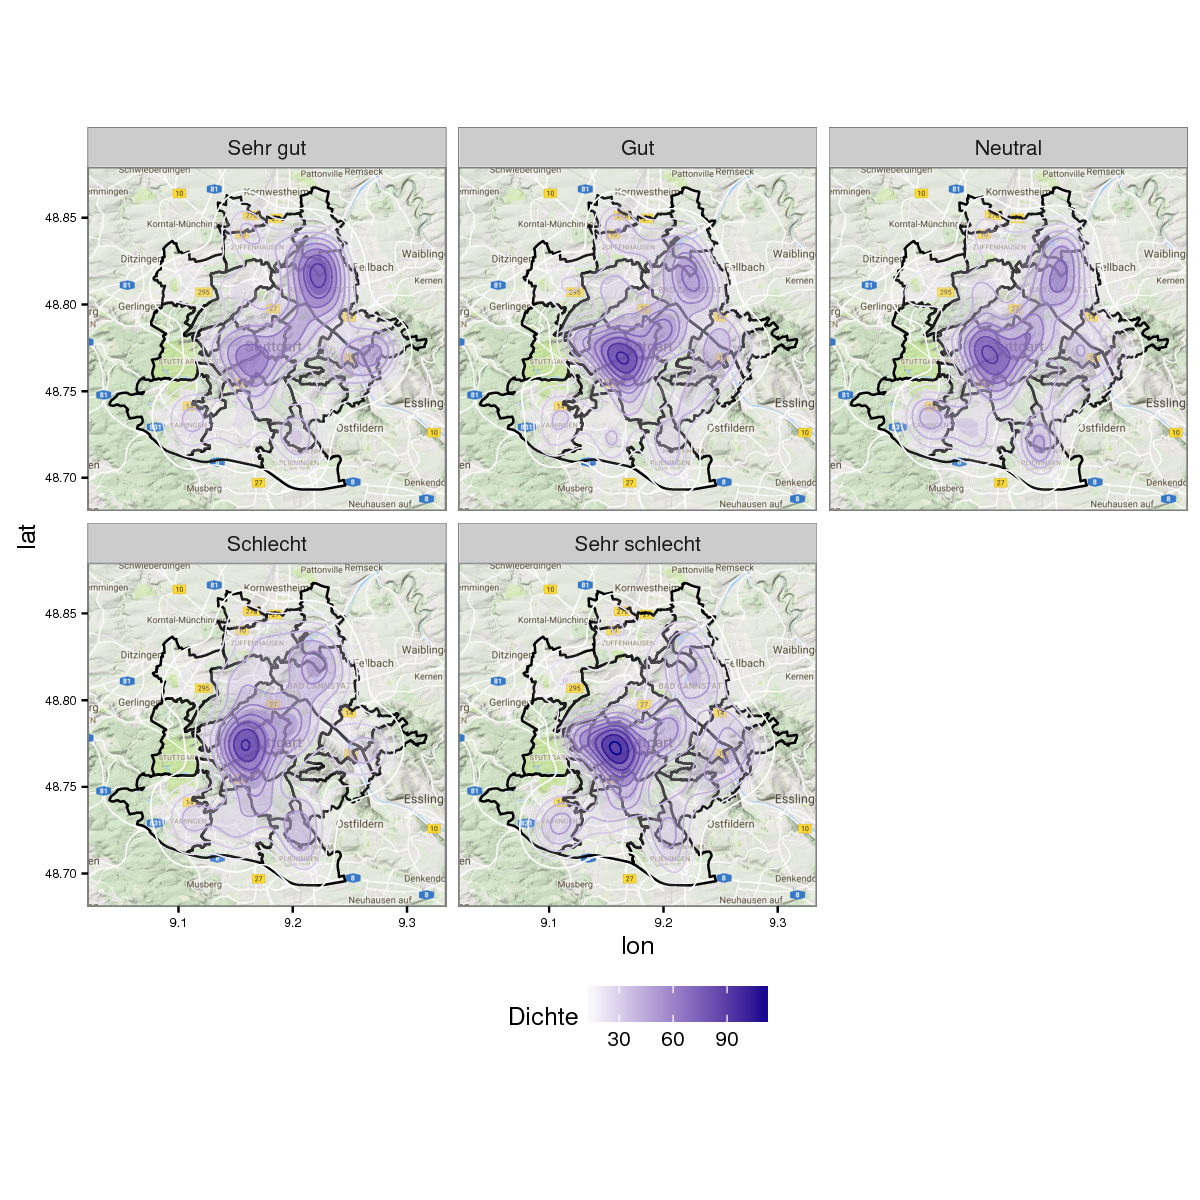
\includegraphics[scale=0.8]{Pictures/XYStuttgart5}
% \caption{Gauss Krüger Informationen Stuttgart 21 (2)}
% \label{endogene}
% \end{center}
%\end{figure}

\end{appendix}
\clearpage
\pagestyle{plain}
%\phantomsection
%\addcontentsline{toc}{section}{Eigenständigkeitserklärung}

%\section{Eigenständigkeitserklärung}

Hiermit versichere ich, dass ich die vorliegende Hausarbeit selbstständig verfasst und keine anderen als die angegebenen
Hilfsmittel benutzt habe. Alle wörtlich oder sinngemäß den Schriften anderer entnommenen Stellen
habe ich unter Angabe der Quellen kenntlich gemacht. Dies gilt auch für beigefügte Zeichnungen, Skizzen, bildliche
Darstellungen und dergleichen.\\
\\
Mir ist bewusst, dass ich mich im Falle einer unbeabsichtigten oder vorsätzlichen Missachtung durch den fehlerhaften
Umgang mit Quellen unter Umständen strafbar mache und die vorliegende Hausarbeit mit nicht ausreichend
bewertet wird.
\\
\\Göttingen, den
\\Unteschrift
\vspace*{4cm}
\\
Hiermit erlaube ich, dass meine Arbeit auf Betrug und falsche, sowie fehlende Zitate auch online geprüft wird.\\
\\
Mir ist bewusst, dass ich mich im Falle einer unbeabsichtigten oder vorsätzlichen Missachtung durch den fehlerhaften
Umgang mit Quellen unter Umständen strafbar mache und die vorliegende Hausarbeit mit nicht ausreichend
bewertet wird.
\\
\\Göttingen, den
\\Unterschrift
\clearpage


\end{document}
